\documentclass[a4paper]{usiinfbachelorproject}

\captionsetup{labelfont={bf}}
%%%%%%%%%%%%%%%%%%%%%%%%%%%% PACKAGES %%%%%%%%%%%%%%%%%%%%%%%%%%%%%
\usepackage{float}
\usepackage{amsmath}

\usepackage{color}
\usepackage{caption}
\usepackage{subcaption}

\usepackage{color}
\usepackage{hyperref}
\hypersetup{
    colorlinks=true,
    linkcolor=black,
    citecolor=black,
    urlcolor=blue,
    linktoc=all
}

\setlength{\parindent}{.3cm}

%%% Main Body %%%

\author{Robert Jans}

\title{\textbf{Experimental Apparatus}}
\subtitle{For a Digital Health Literacy Experiment}
\versiondate{\today}

\begin{committee}
%With more than 1 advisor an error is raised...: only 1 advisor is allowed!
\advisor[Universit\`a della Svizzera Italiana, Switzerland]{Prof.}{Marc}{Langheinrich}
%You can comment out  these lines if you don't have any assistant
\coadvisor[Universit\`a della Svizzera Italiana, Switzerland]{Prof.}{Peter}{Schulz}

\end{committee}

\abstract { 

     In this project we implement a software toolkit for conducting an experiment planned by the \newline
    \emph{Institute~of~Communication~and~Health (ICH)}. The institute is part of the \emph{Faculty of Communication Sciences}
    at the \emph{Universit\`a della Svizzera Italiana}. Health communication is a relatively new and multidisciplinary field, 
    which includes the study and use of communication to inform and affect decision-making at the individual and community 
    level in order to improve the quality of healthcare \cite{ICH_web}. 
    The purpose of the planned experiment is to investigate the digital health literacy of participants in the
    area of sleeping disorders.
    
    This project seeks to provide the experimental apparatus which will allow the research team to record data and test its hypotheses.
    The project's main tasks are indexing a predefined set of websites, creating a user interface similar to common search engines that
    can be configured to selectively show different subsets of the corpus according to the experimental conditions under investigation
    and setting up an experimental environment allowing to conduct controlled experiments and record salient data such as search logs and click-stream.

}
\begin{document}
\maketitle
\tableofcontents\newpage
\listoffigures\newpage

%%%%%%%%%%%%%%%%%%%%%%%%%%%%%%%%%%%%%%%%%%%%%%%%%%
\section{\textbf{Introduction}}
%%%%%%%%%%%%%%%%%%%%%%%%%%%%%%%%%%%%%%%%%%%%%%%%%%

%%%%%%%%%%%%%%%%%%%%%%%%%
\subsection{Motivation}
%%%%%%%%%%%%%%%%%%%%%%%%%

Since the beginning of modern science, researchers have needed special tools in order to conduct experiments. These tools consist 
mainly of devices for taking measurements and triggering phenomena under controlled conditions. Whereas in the past the
experimental apparatuses comprised almost exclusively physical devices, nowadays increasingly more software is involved.
The experiment for which the result of my project is going to be used is a case where the process of 
setting up the experimental conditions and collecting the result data depends heavily on the software toolkit. It is therefore
essential for the software to be robust and reliable.

My personal motivations come from two sides: I have a general interest in science and the scientific method, but in practice,
rather than as a scientist,
I'd see myself as a technician, who in the area of software development seeks to build useful applications.
In that sense, this project perfectly fits my interests, as it involves the creation of software to be used in the context of
scientific research.    

%%%%%%%%%%%%%%%%%%%%%%%%%
\subsection{Outline}
%%%%%%%%%%%%%%%%%%%%%%%%%

\TODO{describe the sections}


%%%%%%%%%%%%%%%%%%%%%%%%%%%%%%%%%%%%%%%%%%%%%%%%%%
\section{\textbf{Requirements}} \label{sec:req}
%%%%%%%%%%%%%%%%%%%%%%%%%%%%%%%%%%%%%%%%%%%%%%%%%%

Below is a description of the requirements as defined by the advisor. The requirements include three main tasks as well 
as eight milestones; the milestones are divided into the categories \emph{must have}, \emph{should have}, and \emph{nice to have}.
While working on the project, some additional requirements were defined, which are described in section 
\ref{sec:reqAdditional}.

%%%%%%%%%%%%%%%%%%%%%%%%%
\subsection{Main Tasks} \label{sec:reqTasks}
%%%%%%%%%%%%%%%%%%%%%%%%%

    \begin{enumerate}

        \item Spidering (i.e. creating a full or partial local copy of) a predefined set of websites that provide
              sleeping disorder information as an experimental corpus. 

        \item Creating a Google-like search interface to the corpus that can be configured to selectively show/rank different sets of
              corpus sites, according to the experimental conditions under investigation.

        \item Setting up an experimental environment (e.g. using the \emph{SafeExamBrowser}, or using a proxy server) to
              conduct controlled experiments using the corpus (e.g. to prevent participants from accessing non-corpus sites)
              and to record salient data (e.g. search logs, click-stream).

    \end{enumerate} 

%%%%%%%%%%%%%%%%%%%%%%%%%
\subsection{Milestones} \label{sec:reqMilestones}
%%%%%%%%%%%%%%%%%%%%%%%%%

    \begin{enumerate}

        \item \textbf{(Must have)} A website simulating a search engine that lets users enter keywords into a search form and
              returns results (including snippets) from a predefined corpus of websites/links, which can then be clicked on / followed.

        \item \textbf{(Must have)} A result generator and a simple way to configure it (e.g. using a text file) on a per-group
              basis (i.e. participants in Group 1 receive results from lists R1, R2, and R3; Group 2 participants
              receive results from R4, R2, and R3).

        \item \textbf{(Must have)} A report describing the system's installation, setup, and architectural design. 

        \item \textbf{(Should have)} A result generator that can detect identical, repeated queries (or minor variations of
              otherwise identical queries, detectable via stop word removal and stemming) upon which it will generate the same response.

        \item \textbf{(Should have)} A detailed log engine that allows the experimenter to track key experimental results
              for each participant, such as search terms entered, the time spent on a given result list, and any clicks on
              results (when, which order).

        \item \textbf{(Should have)} A visual presentation of the search entry and result section that mimics a known search engine.  

        \item \textbf{(Nice to have)} A result generator that can handle non-related searches using a pass-through to a real search engine.

        \item \textbf{(Nice to have)} A web interface to the log engine that allows for convenient inspection, analysis,
              and export of experimental results.

    \end{enumerate}

%%%%%%%%%%%%%%%%%%%%%%%%%
\subsection{Additional Requirements} \label{sec:reqAdditional}
%%%%%%%%%%%%%%%%%%%%%%%%%

\begin{itemize}

    \item It must be possible to embed the application into a survey created using the \emph{Qualtrics} platform \cite{qualtricsHome}. 

    \item Instead of linking directly to the original web page, a click on an item in the search result list should lead
to a page containing its own navigation bar, so users can easily return to the search interface.

    \item As a result for the first query, all participants will receive the same predefined result list (configurable per
test group). Only subsequent queries will be processed by the search engine.

\end{itemize}

%%%%%%%%%%%%%%%%%%%%%%%%%%%%%%%%%%%%%%%%%%%%%%%%%%
\section{\textbf{Project Design}} \label{sec:design}
%%%%%%%%%%%%%%%%%%%%%%%%%%%%%%%%%%%%%%%%%%%%%%%%%%

%%%%%%%%%%%%%%%%%%%%%%%%%
\subsection{General Structure} \label{sec:designGeneral}
%%%%%%%%%%%%%%%%%%%%%%%%%

Given the close relationships between the experiment configuration, conduction, and analysis, I decided to include
most of the implied functionalities into a single web application, called \emph{HSE (Health Search Engine)}.
The user management functionality of HSE allows participants to access only a search interface, while experimenters
have access to pages for managing corpora and experiments. If needed, participants can be prevented from
accessing non-corpus sites by restricting the browser to a whitelist based on the corpus used for a given experiment.
The following subsections briefly describe the usage modalities and the related user interfaces.

%%%%%%%%%%%%%%%%%%%%%%%%%
\subsection{Typical Usage Workflow} \label{sec:designWorkflow}
%%%%%%%%%%%%%%%%%%%%%%%%%

The typical workflow includes four steps: preparing the document corpora, setting up an experiment, running the experiment,
and finally evaluating the resulting data. \textbf{Figure \ref{fig:usage}} shows this usage scenario. 
To each step corresponds a dedicated user interface. 

For preparing the corpora the experimenter provides text files containing the web URLs of the chosen documents. After setting the names for the
corresponding document collection, the application takes care of downloading the contents and creating the inverted indices needed for retrieval.
Setting up an experiment involves defining test groups and assigning participants to each group. Moreover, for each test group, it is needed
to set the document collections from which the retrieval mechanism will select the results to be displayed to the participants.
The groups can be defined either manually or by uploading a configuration file.
The U.I. for experiment execution includes a control button for starting, stopping, or resetting an experiment, as well 
as a tabular display for real-time monitoring, showing the current number of queries and clicks for each participant.
Starting an experiment enables the participants to log in, and initiates the data collection mechanism; after
stopping the experiment, the participants are logged out, and transient data is saved.
The experiment evaluation interface  allows for quick inspection through data summaries and visualizations. Moreover, it allows
exporting both the raw data and the summaries as files.

\begin{figure}[h]
\centering
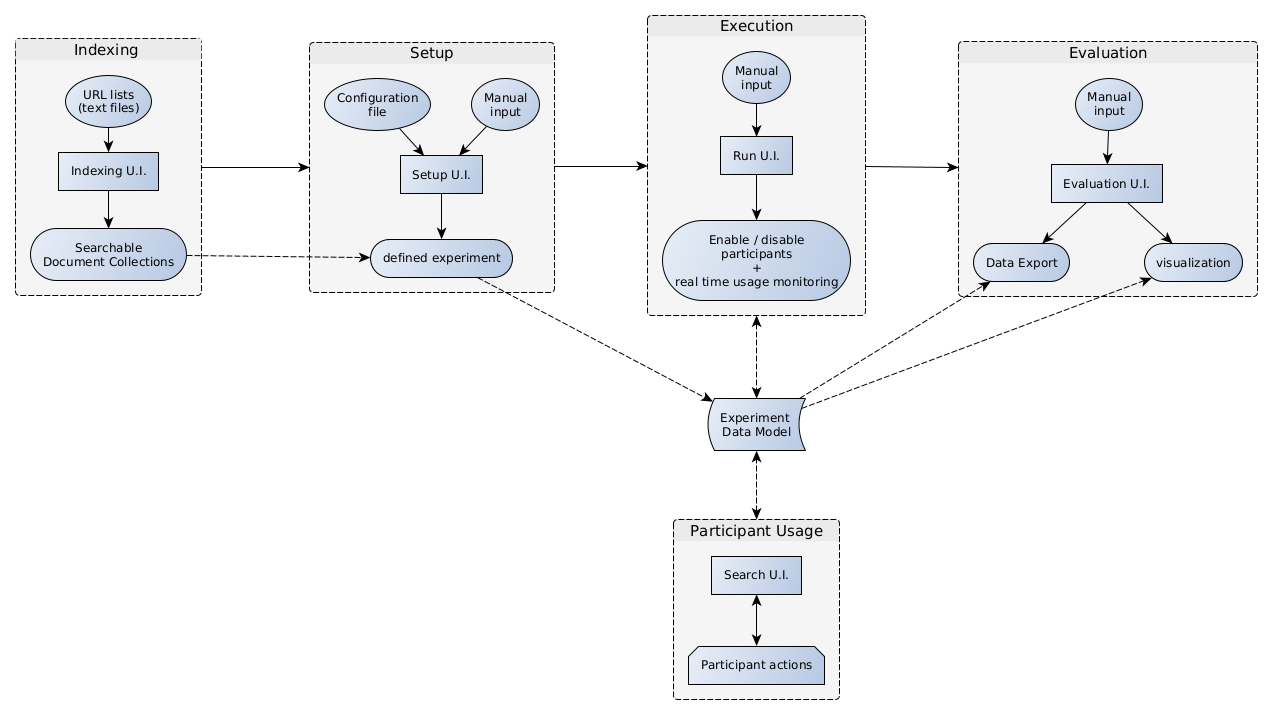
\includegraphics[width=0.7\textwidth]{figures/usage}
\caption{Typical usage workflow}
\label{fig:usage}
\end{figure}


%%%%%%%%%%%%%%%%%%%%%%%%%
\subsection{Defining the Document Corpora} \label{sec:designDefineDocs}
%%%%%%%%%%%%%%%%%%%%%%%%%

In order to define the document collections (corpora) to be used during subsequent experiments, 
an experimenter can upload text files containing lists of web URLs. The files are  stored, so they can be reused 
for defining multiple document collections. Via a popup menu, a new  document collection can be defined by providing a name, 
the collection's language, and the related URL list.
Clicking on the ``index'' button initiates the indexing process, which includes data download and the creation of an index
data structure for retrieval. The details of the indexing process are explained in section \TODO{link actual section}.
\textbf{Figure \ref{fig:indexing}} shows the relevant parts of the interface.

\begin{figure}[h]
     
     \centering
     \begin{subfigure}[b]{0.6\textwidth}
         \centering
         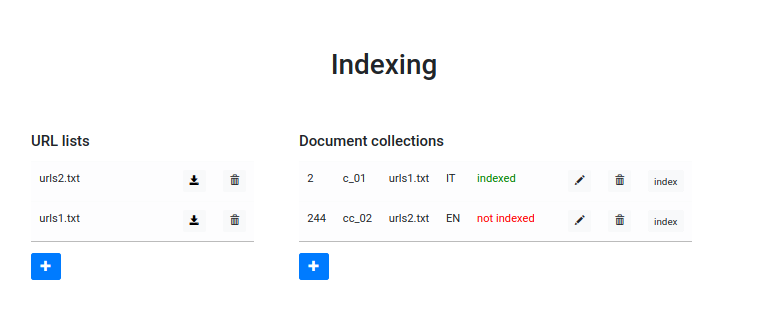
\includegraphics[width=.8\linewidth]{figures/indexing1}
         \caption{indexing  u.i}
         \label{fig:indexingA}
     \end{subfigure}
     \begin{subfigure}[b]{0.3\textwidth}
         \centering
         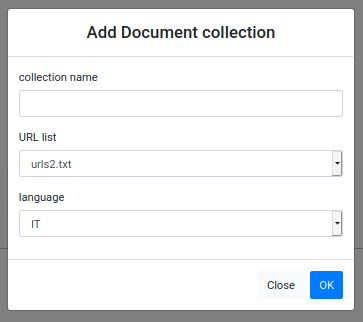
\includegraphics[width=.6\linewidth]{figures/indexing2}
         \caption{popup for defining  document collections}
         \label{fig:indexingB}
     \end{subfigure}
     \caption{Indexing UI page}
     \label{fig:indexing}

\end{figure}


%%%%%%%%%%%%%%%%%%%%%%%%%
\subsection{Setting up an Experiment} \label{sec:designExpSetup}
%%%%%%%%%%%%%%%%%%%%%%%%%

The UI for experiment setup allows defining the details of an experiment to be carried out. This step involves creating
test groups with associated participants and document collections. Groups can be defined either manually or by using 
an uploaded configuration file. In both cases, the test group configuration can later be edited manually. 
The interface allows linking each group to a set of previously indexed document collections. Optionally a document collection
can be set for each test group as predefined result list to be returned after the the first query.
If the experiment is to be executed in the context of a \emph{Qualtrics} survey, the participants don't need to be specified, as they are
defined while they take part in the survey. 
\textbf{Figure \ref{fig:setup}} shows this UI.

\begin{figure}[h!]
\centering
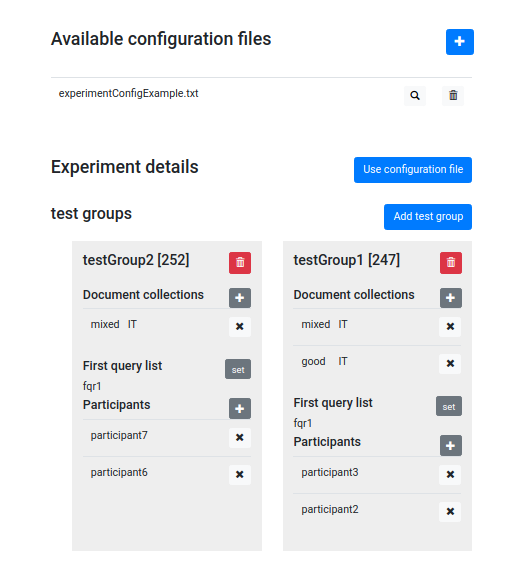
\includegraphics[width=0.6\textwidth]{figures/setup}
\caption{U.I. for experiment setup}
\label{fig:setup}
\end{figure}


%%%%%%%%%%%%%%%%%%%%%%%%%
\subsection{Running an Experiment} \label{sec:designExpRun}
%%%%%%%%%%%%%%%%%%%%%%%%%

The UI for experiment execution includes a start/stop/reset button, a timer, and a tabular display 
showing the current participant activities. Clicking the start button starts the timer, enables the participants to log in, and
initiates the data collection process. While the experiment is running, all queries and click carried out by the
participants are stored as database records including a timestamp, user id, group id, and query/document related data.
The details of the data collection mechanism are described in section \ref{sec:data}.
When the stop button is clicked the participants are logged out and all transient data is saved to the database.
After the experiment is complete the related evaluation page becomes available.
In case something goes wrong, the experiment can be reset. This causes all collected data to be deleted, while the
experiment's configuration is preserved.
\textbf{Figure \ref{fig:run}} shows the user interface.

\begin{figure} [h]
\centering
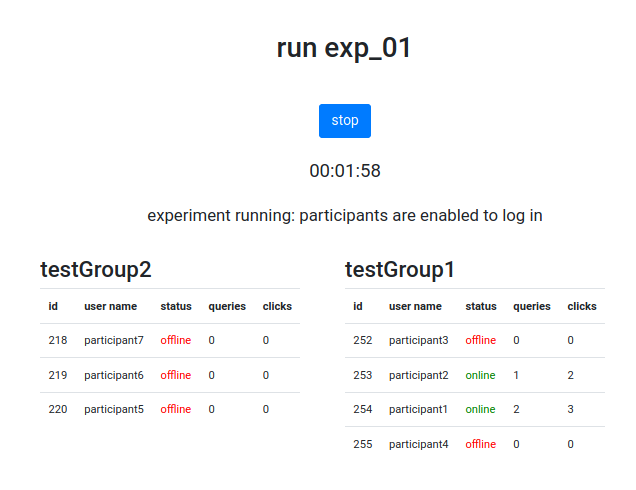
\includegraphics[width=0.6\textwidth]{figures/run}
\caption{UI for experiment execution}
\label{fig:run}
\end{figure}

%%%%%%%%%%%%%%%%%%%%%%%%%
\subsection{Search Interface Available to Participants} \label{sec:designSearchUi}
%%%%%%%%%%%%%%%%%%%%%%%%%

The interface available to the participants looks similar to the main page of most known search engines. It simply
includes a search text bar and a button for entering queries and displays the results as a list of
links accompanied by short summaries (snippets) with highlighted query terms. 
\textbf{Figure \ref{fig:searchUi}} shows the UI after a query has been entered.

\begin{figure} [h]
\centering
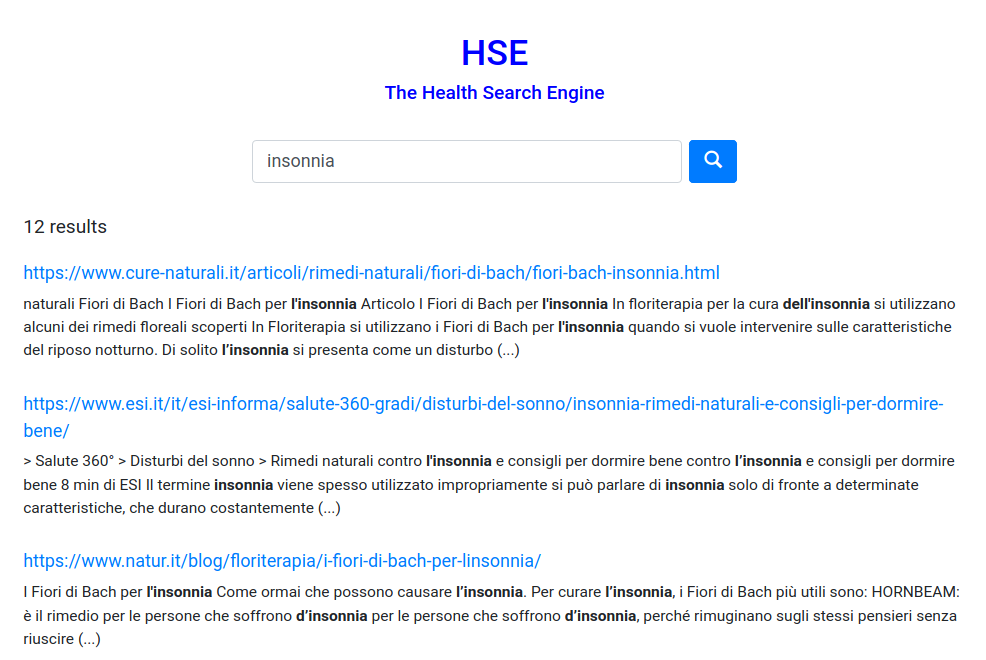
\includegraphics[width=0.7\textwidth]{figures/searchUi}
\caption{User interface available to participants}
\label{fig:searchUi}
\end{figure}

%%%%%%%%%%%%%%%%%%%%%%%%%
\subsection{Experiment Evaluation} \label{sec:designExpEval}
%%%%%%%%%%%%%%%%%%%%%%%%%

After an experiment has been conducted, the  related evaluation interface becomes available. From this page,
experimenters can inspect the experiment's results and export  the complete raw data
or preprocessed data summaries.

The raw data can be exported either in \emph{CSV} or \emph{JSON} format and consists of a list of all user actions that occurred during the experiment. 
Each record has a timestamp, a user id, and a group id. Query event records include the query text and the proportions in which
the data collections are represented  in the result list. Document click event records include the document id, its URL, and
the collection to which the given document belongs.

The data summaries include overall experiment statistics and per-group statistics. Moreover, the individual user histories can be 
exported in the same formats as the raw data.
Per-experiment statistics include the total count of clicks and queries as well as averages, medians, and standard deviations
for queries per user, clicks per user, clicks per query, time per query, and time per click.
Per group statistics include the same metrics as the per-experiment statistics, plus totals, averages, medians, and standard deviations
for clicks per document collection. Details on the raw data format and the computed statistics are described in \ref{sec:data}.

%%%%%%%%%%%%%%%%%%%%%%%%%%%%%%%%%%%%%%%%%%%%%%%%%%
\section{\textbf{Raw Data Generation and Computed Statistics}} \label{sec:data}
%%%%%%%%%%%%%%%%%%%%%%%%%%%%%%%%%%%%%%%%%%%%%%%%%%

%%%%%%%%%%%%%%%%%%%%%%%%%
\subsection{Raw Data Records} \label{sec:dataRaw}
%%%%%%%%%%%%%%%%%%%%%%%%%

The usage tracking system is based on generating records whenever a participant performs a relevant action. The application
distinguishes three kinds of usage events: session events (log in / log out), query events (generated when a participant
submits a search query), and document click events (generated when a participant visits a page by clicking on an item in the search results list). All usage events include the following data fields:

    \begin{itemize}

        \item
        A unique id.

        \item
        A timestamp indicating the precise time when the event occurred.

        \item
        The id of the participant who triggered the event.

        \item
        The id and name of the test group which the participant belongs to.

        \item
        The event type (one of ``SESSION'', ``QUERY'', or ``DOC\_CLICK'').


    \end{itemize}

Query events contain the following additional fields:

    \begin{itemize}

        \item
        The query string entered by the participant.

        \item
        The total number of results retrieved.

        \item
        The number of results retrieved from each of the available document collections.

    \end{itemize}

Document click events contain the following additional fields:

    \begin{itemize}

        \item
        The URL of the corresponding web page.

        \item
        The document's id assigned during indexing.

        \item
        The id and name of the document collection the given document belongs to.

        \item
        The document's rank (i.e. its position within the search results list).


    \end{itemize}

The raw data records can be exported via the experiment's evaluation page in \emph{CSV} or
\emph{JSON} format in order to be used for statistical analysis. Some basic metrics are
computed by the application, as described in the following subsection, and displayed on the
evaluation page.

%%%%%%%%%%%%%%%%%%%%%%%%%
\subsection{Computed data} \label{sec:dataPerExperiment}
%%%%%%%%%%%%%%%%%%%%%%%%%

For each experiment the following quantities are considered:

    \begin{itemize}

        \item
        The total number of query events occurred.

        \item
        The total number of document click events occurred.

        \item
        Mean, median and standard deviation of the number of queries per user.

        \item
        Mean, median and standard deviation of the number of document clicks per user.

        \item
        Mean, median and standard deviation of the number of clicks per query.

        \item
        Mean, median and standard deviation of the time spent per document \\ (duration between a document click event and the next usage event performed by the same participant)

        \item
        Mean, median and standard deviation of the time spent per query \\ (duration between a query and the next query or logout).

    \end{itemize}

The same metrics are available for each test group, allowing for interesting comparisons. Moreover, for each test group, the distribution
of documents visited and time spent over the document collections from which the results are drawn is represented.
Section \ref{impl:dataSummaries} describes the details of how these measures are computed.

%%%%%%%%%%%%%%%%%%%%%%%%%%%%%%%%%%%%%%%%%%%%%%%%%%
\section{\textbf{Software Architecture and Employed Frameworks}} \label{sec:arch}
%%%%%%%%%%%%%%%%%%%%%%%%%%%%%%%%%%%%%%%%%%%%%%%%%%

The project requirements implied building a web application including a text information retrieval system. Both aspects are highly complex and it would not be reasonable to build such an application completely from scratch, so I
needed to rely on appropriate libraries and frameworks. As general framework I chose \emph{SpringBoot}, since
I had used it in past projects and knew that it includes very useful features for handling the main issues related to
serving web pages, interacting with a database, and providing endpoints for \emph{Ajax} calls and \emph{WebSocket} services.
For the information retrieval part, I chose \emph{Apache Lucene}, which includes all functionalities needed for indexing and retrieval,
and since it is a \emph{Java} library, it can be easily integrated into a \emph{SpringBoot} application. As a database management system
I chose \emph{MySql}, but I could have chosen any similar tool.

%%%%%%%%%%%%%%%%%%%%%%%%%
\subsection{SpringBoot: a Java framework for web applications} \label{sec:archSpring}
%%%%%%%%%%%%%%%%%%%%%%%%%

%%%%%%%%%%%%%%%%%%%%%%%%%
\subsection{Lucene: an Open Source Information Retrieval Library} \label{sec:archLucene}
%%%%%%%%%%%%%%%%%%%%%%%%%

%%%%%%%%%%%%%%%%%%%%%%%%%
\subsection{Back-end Code Organization} \label{sec:archBackend}
%%%%%%%%%%%%%%%%%%%%%%%%%

%%%%%%%%%%%%%%%%%%%%%%%%%%%%%%%%%%%%%%%%%%%%%%%%%%
\section{\textbf{Implementation details}} \label{sec:impl}
%%%%%%%%%%%%%%%%%%%%%%%%%%%%%%%%%%%%%%%%%%%%%%%%%%

%%%%%%%%%%%%%%%%%%%%%%%%%
\subsection{User Management} \label{impl:users}
%%%%%%%%%%%%%%%%%%%%%%%%%

%%%%%%%%%%%%%%%%%%%%%%%%%
\subsection{Data Extraction and Summary Generation} \label{impl:dataSummaries}
%%%%%%%%%%%%%%%%%%%%%%%%%


%%%%%%%%%%%%%%%%%%%%%%%%%%%%%%%%%%%%%%%%%%%%%%%%%%
\section{\textbf{Under the Hood: The Information Retrieval Process}} \label{sec:ir}
%%%%%%%%%%%%%%%%%%%%%%%%%%%%%%%%%%%%%%%%%%%%%%%%%%


\newpage
	
%%%%% BIBLIOGRAPHY %%%%%
\bibliographystyle{abbrv}
\bibliography{references}

\end{document}





















